\chapter{Results and Discussion}\label{chap:chap5}

\section*{}

\section{Introduction}

Generally, the first objective a developer has when building software is making it work. After some experience and good practices, the development becomes faster, elegant and with concerns about its performance. When dealing if performance issues, there is a lot of measures to pay attention from the lowest hardware level to the highest software level. Now-a-days performance is as much important as the creating software, because it makes the work faster, with less cost, and, in the end, more revenue. However it is really hard for a single person masters performance as a whole because there are to many variables, conditions, aspects, and realities making humanly impossible mastering everything.

The approach to achieve high performance level is to have handful of expertises in each concrete area. Even so, mastering specific fields in the performance level, it is hard, takes time, lots of effort and most of the times impossible to achieve the perfect performance. Since achieving high level of performance is so important and requires a lot of effort to try to achieve it, then, first of all, is it possible to achieve high performance level in applications in an automatic way? If so, how can it be achievable? Can it totally replace an expert?

Focusing these question to the field of code parallelization, more will rise, not necessarily related to this specific filed: since exists tools, like Kremlin, which help to, automatically, parallelize code, how acceptable are their results? How this specific tool can help in getting one step closer to automatic code parallelization? In which way can Kremlin be better than an expert?

In order to answer all previous questions, this chapter is divided in two main sections: the first section is related to the Kremlin's activity and how is it helpful. The second section is the confrontation of all the gathered data to verify what is better and how can it contribute to the future of automatic code parallelization. 


\section{Kremlin's reports}

When Kremlin compiles and profiles a sequential code, it provides a report with locations of the blocks that can be parallelized. Additional it gives some values that indicates the theoretical gain if the parallelization is implemented.

For the \textit{Mult} and \textit{MultLine} algorithm, Kremlin gave these reports~\ref{report:onmulkremlin}~\ref{report:onmulinekremlin}, respectively. Taking into account that the manual code parallelization was done in the first place, the risk of being bias is null and, additionally, helps to understand if Kremlin is reporting things correctly.

In this case, Kremlin detected the block code with the most impact on application performance for both implementations (\textit{Mult} and \textit{MultLine}). Additionally, Kremlin's report pointed the locations of more blocks to be parallelized, however, the impact of these blocks being parallelised might have a low impact on applications' performance, also for both implementations. The impact of the parallization made in the others block is analysed in the next section because a verdict can be made after comparing the execution times of the Manual's group against Kremlin's group. 

The justification behind these analysis is based on the \textit{ time reduced}, \textit{ideal time reduced}, \textit{coverage} and \textit{self parallelism} values and the block location, provided by the report, comparing with the expected result and manual code parallelization by an expert, in both implementation.

Getting a close look in these reports, at the left side is \textit{Mult} report values,~\ref{report:onmulkremlin}, and on the right side is \textit{MultLine} report values,~\ref{report:onmulinekremlin}:

\begin{table}[htb]
\centering
\caption{Kremlin's report values for the matrix multiplication block}
\begin{tabular}{ |l|l| }
	\hline
	\textbf{Time reduced} & 66.38\% \\ \hline
	\textbf{Ideal time reduced} & 70.96\% \\ \hline
	\textbf{Coverage} & 88.51\% \\ \hline
	\textbf{Self parallelism} & 5.05 \\
	\hline
\end{tabular}
\quad
\begin{tabular}{ |l|l| }
	\hline
	\textbf{Time reduced} & 63.01\% \\ \hline
	\textbf{Ideal time reduced} & 63.20\% \\ \hline
	\textbf{Coverage} & 84.02\% \\ \hline
	\textbf{Self parallelism} & 4.03 \\
	\hline
\end{tabular}
\end{table}

In both reports, the high percentage of the reduced time and time reduced means that parallelizing these blocks the execution time of this block is, theoretically, reduced in between those two values. 

Taking a close look in the others blocks, their locations refers to the matrices initialization and the values of timed reduced and ideal timed reduced are really low, around 3\% in both implementations, which means that the improved performance is insignificant and might cause delay in during de applications executions. However, this situations is confirmed in the next section. 


\section{Comparison between Original, Manual and Kremlin}

The previous section has an important role because the reports credibility and correctness influences the the results in this chapter, consequently, could lead to misguided and wrong conclusions. Since the report gave correct feedback and it is well justified, the following values are valid.

To get a satisfying answer for the initial questions, it is necessary to, in first place, understand context of each experience and respective results; following the evolution and the comparison is made between data. So, in a first instance, each group (Original, Manual, Kremlin) is going to be analysed individually to stablish the context and basis knowledge. Then, the second subsection will focus in measuring the impact of Manual and Kremlin group have to the Original group to prove that these measures, in practical terms, have a huge impact improving applications performance. After this knowledge also as been established, the results will prove if the Kremlin's guidelines make the code with better performance comparing to the expert's results parallelizing the code manually, and respond to the question if  automaticly parallelizing code is a reliable and good practice.

\subsection{The Three groups individually analysed}

As mentioned in the previous chapter, each group has its purpose
based on the variables used and results obtained. To understand the overall impact of these implementations, it is important to firstly understand the experiences that were made in each group separately and analyse their results, step by step.

\subsubsection{Original}

This group has the sequential code version of the \textit{Mult} and \textit{MultLine} algorithms. As mentioned earlier, this group stablish the base reference for the execution time. From now on, all experiences should have better performance, unless there is an explanation for the Original Group has better results, in some particular cases.

\begin{figure}[htb]
	\begin{center}
		\leavevmode
		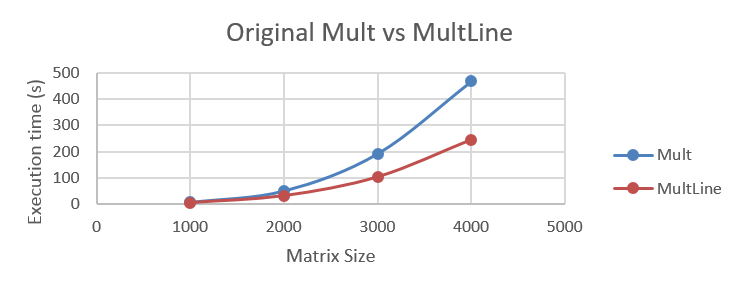
\includegraphics[width=0.8\textwidth]{original}
		\caption{Dispersion plot that represents the evolution of execution time with the matrix size increase in both \textit{Mult} and \textit{MultLine} sequential implementations}
		\label{fig:original}
	\end{center}
\end{figure}

According to Figure~\ref{fig:original}, the \textit{MultLine} algorithm has better results the higher the matrix size is, as expected, since this algorithm takes advantage of the values preloaded in memory cache.

Another aspect noteworthy is the increase of the function inclination variation, in both implementations, as the matrix size increases. Specially for the  \textit{Mult} implementation. This is related to the memory cache size. The smaller the size the higher will be de variation of the function inclination.

\subsubsection{Manual}\label{subsubsec:manual}

Manually parallelizing a code requires a lot of effort, time and know-how since the way it is done requires de expert to understand the code, have practice in detecting potential parallelized blocks of code, identify the best way to parallelize those blocks and test the work until it gives a reasonable result.
So, this group corresponds to this situation and, in theoretical perspective, has the bests results. 

\begin{figure}[htb]
	\begin{center}
		\leavevmode
		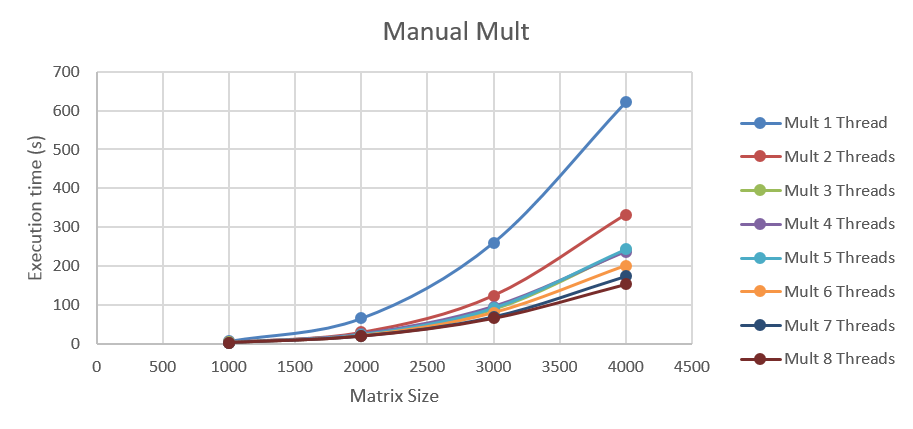
\includegraphics[width=0.9\textwidth]{manualmul}
		\caption{Dispersion plot that represents the evolution of execution time with the matrix size increase in function of the number of threads. Version of the manual code parallelization for \textsl{Mult} algorithm}
		\label{fig:manualmul}
	\end{center}
\end{figure}

\begin{figure}[htb]
	\begin{center}
		\leavevmode
		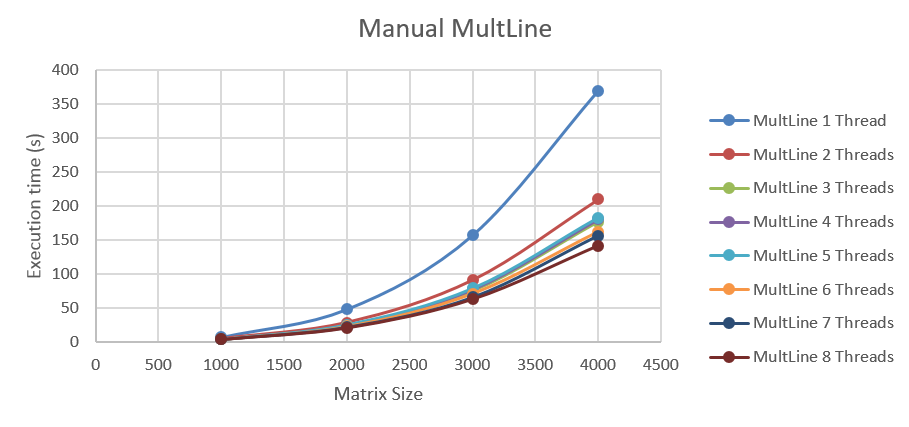
\includegraphics[width=0.9\textwidth]{manualmuline}
		\caption{Dispersion plot that represents the evolution of execution time with the matrix size increase in function of the number of threads. Version of the manual code parallelization for \textsl{MultLine} algorithm}
		\label{fig:manualmuline}
	\end{center}
\end{figure}

Figure~\ref{fig:manualmul} and Figure~\ref{fig:manualmuline} have similar behaviours including the fact that using eight threads makes the application with the best performance because the executed time is inferior as long as the matrix size increases.

\begin{figure}[htb]
	\begin{center}
		\leavevmode
		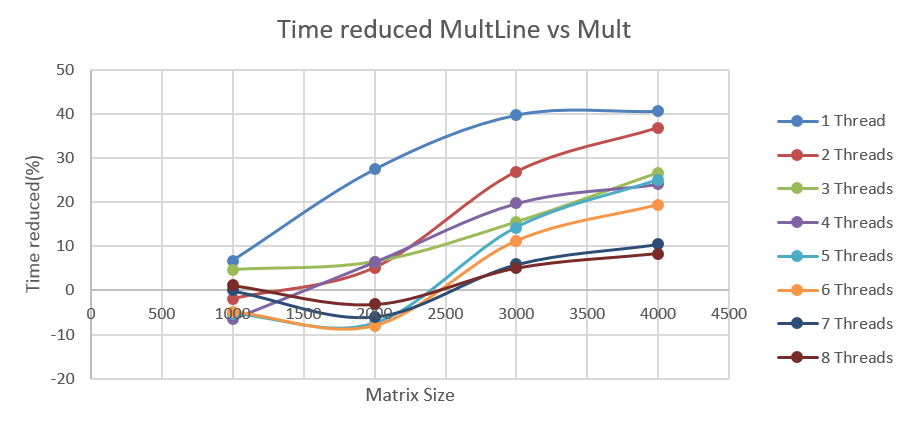
\includegraphics[width=1\textwidth]{manualreducedtime}
		\caption{Dispersion plot that represents the evolution of time reduced with the matrix size in function of the number of threads. Versions of \textit{Mult} and \textit{MultLine} manual implementations. }
		\label{fig:manualreducedtime}
	\end{center}
\end{figure}

However, there is a difference between these two plots is the value of the execution time. This difference can be analysed in Figure~\ref{fig:manualreducedtime}. Time reduced is a percentage of how much the \textit{MultLine} implementation reduces comparing to the \textit{Mult} implementation. 

It is a fact, observed in Figure~\ref{fig:manualreducedtime}, that increasing the matrix size, the time reduced tends to a certain value which is independent of the number of threads. This value is the ceiling where \textit{MultLine} algorithm can not be better than \textit{Mult} algorithm for the same hardware components; meaning the existence of a hardware limitation (processor power, memory ram and cache size) since the increase of the matrix size will, proportionally, increase the number of loads, writes and cache missed for both algorithms.

Another fact is that the higher the thread number, lesser will be de timed reduced, and lesser will be the executed time, also related to the maximum capacity of threads a multi-core processor can have and have working at the same time.

Another noteworthy fact is , for low values of matrix size, 1000 and 2000, and the higher the number of threads being used, the time reduced is negative, meaning executed time for \textit{Mult} implementation is lower than \textit{MultLine} implementations, concluding that  \textit{Mult} implementation is better suited for low size data in case a high number of threads are being used. This is due to many threads are being used simultaneously and they are trampling each other in order to complete their task, which increases the overall overhead, and so the reason behind ne time reduced negative value.


\subsubsection{Kremlin}

This group is constituted by the result of the implementations indicated by Kremlin's report. The experiences conducted in this group and the respective obtained results will demonstrate if Kremlin can actually bring acceptable results. 

\begin{figure}[htb]
	\begin{center}
		\leavevmode
		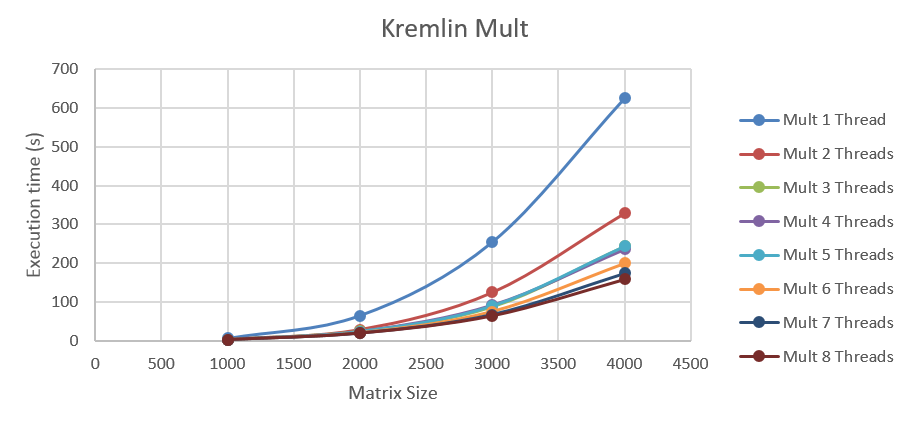
\includegraphics[width=0.9\textwidth]{kremlinmul}
		\caption{Dispersion plot that represents the evolution of execution time with the matrix size increase in function of the number of threads. Version of the Kremlin code parallelization for \textsl{Mult} algorithm}
		\label{fig:kremlinmul}
	\end{center}
\end{figure}

\begin{figure}[htb]
	\begin{center}
		\leavevmode
		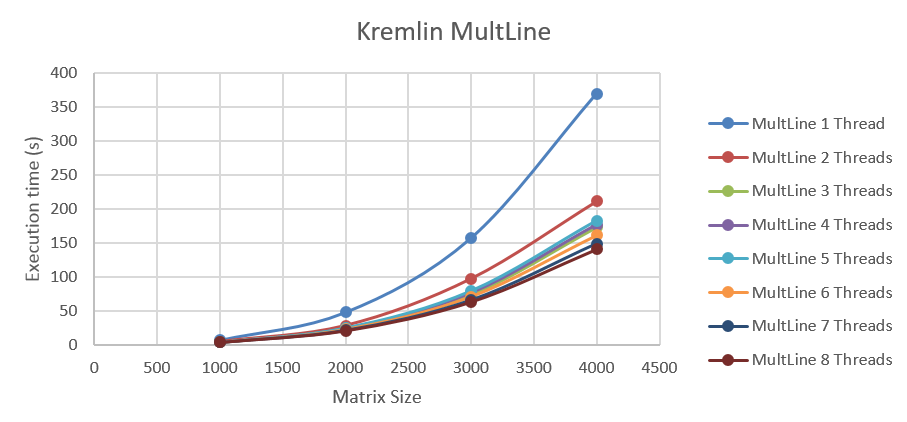
\includegraphics[width=0.9\textwidth]{kremlinmuline}
		\caption{Dispersion plot that represents the evolution of execution time with the matrix size increase in function of the number of threads. Version of the Kremlin parallelization code for \textsl{Multline} algorithm}
		\label{fig:kremlinmuline}
	\end{center}
\end{figure}

Figure~\ref{fig:kremlinmul} and Figure~\ref{fig:kremlinmuline}, as expected, have similar behaviour compared to manual group, since the code samples from both groups have the same structure and the experimental environment is the same: same experimental variables(matrix size, number of threads, parallelized code) and same result type (execution time).

\begin{figure}[htb]
	\begin{center}
		\leavevmode
		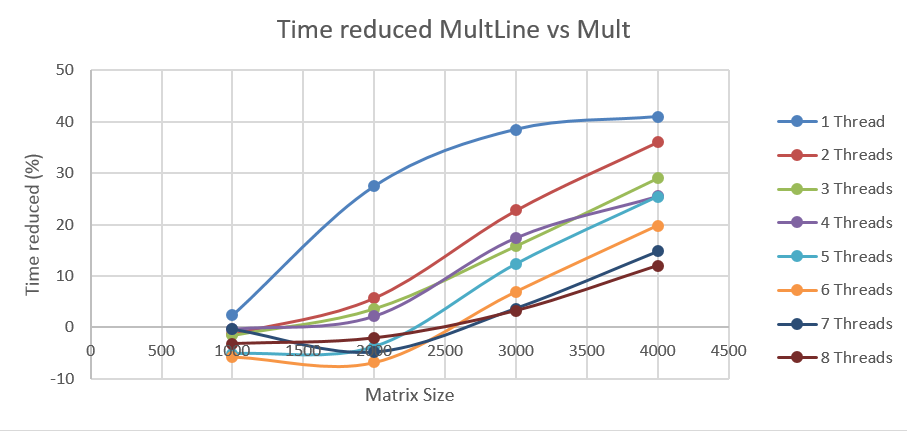
\includegraphics[width=0.9\textwidth]{kremlinreducedtime}
		\caption{Dispersion plot that represents the evolution of time reduced with the matrix size in function of the number of threads. Versions of \textit{Mult} and \textit{MultLine} Kremlin's implementations.}
		\label{fig:kremlinreducedtime}
	\end{center}
\end{figure}

Additionally, and for the same reason, Figure~\ref{fig:kremlinreducedtime} also has the same behaviour has the manual group and, therefore, the analysis is the same.

\subsubsection{Overall review}

Through the analysis of these three tests groups, separately, and since these groups were tested under the same circumstances, it is possible to conclude that using these versions of the matrix multiplication algorithm do not jeopardize the results, since they have similar behaviours, moreover, they increase assurance and credibility for the following up analysis and conclusions. It is because of the similarity of behaviours that this comparison is valid and correct, even so the performance is different, which was expected, as explained before.

\subsection{Measuring the performance's impact using code parallelization}

The conducted analysis presented in previous section explains the characteristics of each group and the plausible connection with each other. To quantify how beneficial can code parallelization be, the next sub sub sections will prove its impact. 

The first sub sub section compares how much better was the improvement for Manual group, using the Original group as base. The second sub sub sections compares the same ways as the previous sub sub sections but, instead using the Manual group, it will be the Kremlin group. Finally, overall conclusions will be presented about both sub sub sections. 

For this analysis, either Manual or Kremlin groups, the number of threads that will be used is eight since, and for both groups, using eight threads gave the best performance results. This does not mean that for the other number of threads the results were worst than the Original group, far from that. The goal is achieving the highest performance, so the best results were picked.

\subsubsection{Comparison between Manual and Original groups}

In Figure~\ref{fig:manualoriginal} is presented a dispersion plot 
demonstrating that Manual group has an overwhelming better performance and that performance increases with the matrix size to a certain point, explained in~\ref{subsubsec:manual}. This includes both implementations.
\begin{figure}[htb]
	\begin{center}
		\leavevmode
		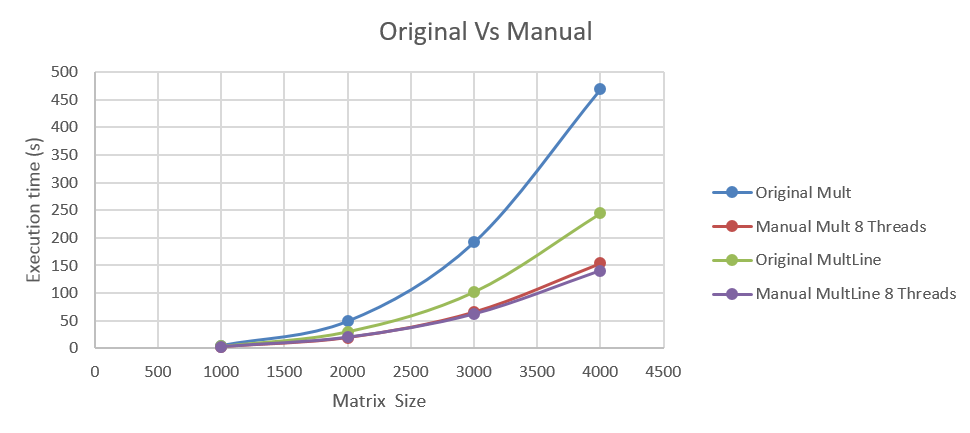
\includegraphics[width=0.8\textwidth]{manualoriginal}
		\caption{Dispersion plot that represents the evolution of execution time with the matrix size in function of Manual and Original.}
		\label{fig:manualoriginal}
	\end{center}
\end{figure}

With this plot. it is proved that using parallelization techniques in programs and applications can achieve higher performances. In this particular case, it can be more than twice better for the \textit{Mult} case and almost twice for \textit{MultLine}. These values are presented in ~\ref{subsubsec:overall}.

\subsubsection{Comparison between Kremlin and Original groups}

Regarding the Kremlin experimental results, in Figure~\ref{fig:kremlinoriginal} is shown a dispersion plot revealing, as expected, and like in the previous sub sub section, that Kremlin's group surpassed the Original group in terms of execution time, in both implementations.

\begin{figure}[htb]
	\begin{center}
		\leavevmode
		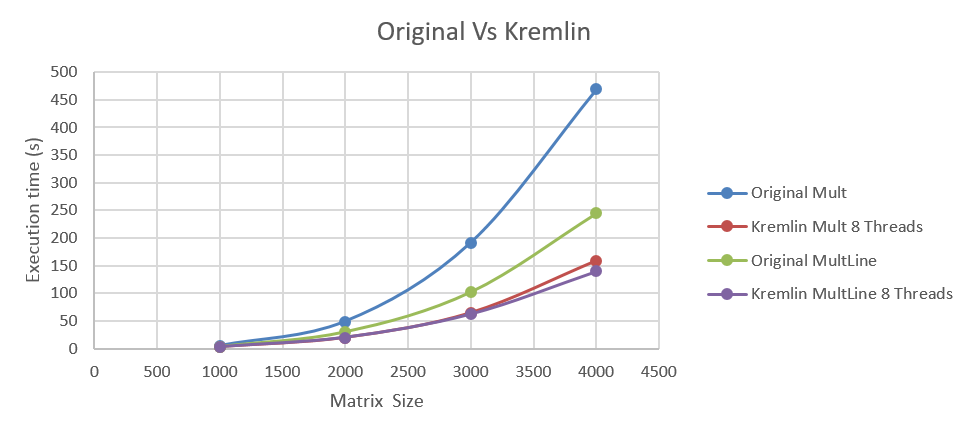
\includegraphics[width=0.8\textwidth]{kremlinoriginal}
		\caption{Dispersion plot that represents the evolution of execution time with the matrix size in function of  Kremlin and Original groups implementations.}
		\label{fig:kremlinoriginal}
	\end{center}
\end{figure}

Like in previous case, this plot proves that using Kremlin as an automatic tool to help identifying parallelizable code blocks can enhance applications performance and is a good asset because it can save time by indicating where it is possible to make a block parallel, instead of the developer looking for them.

\subsubsection{Overall comparison}\label{subsubsec:overall}

If code parallelization would not bring any beneficial impact in programs and applications, obviously, it would make no sense using it. Additional, and for this concrete case, if Kremlin's performance was worst, this tool would be useless to help in making paralleled code automatically, and the test would and here.


\begin{figure}[htb]
	\begin{center}
		\leavevmode
		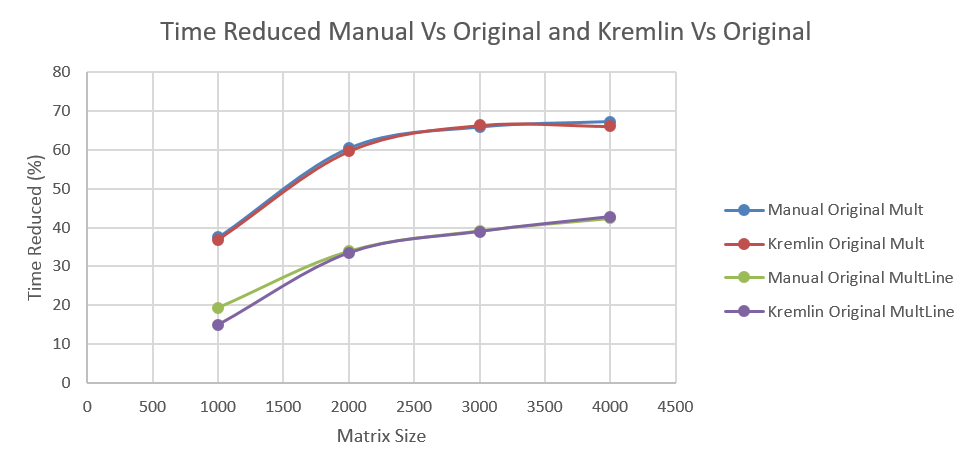
\includegraphics[width=1.1\textwidth]{reducedtimeall}
		\caption{Dispersion plot that represents the evolution of time reduced with the matrix size in function of Manual and Kremlin groups implementations.}
		\label{fig:reducedtimeall}
	\end{center}
\end{figure}

In Figure~\ref{fig:reducedtimeall} is compared the time reduced for Manual and Kremlin groups comparatively to Original Group. From this plot it is drawn that \textit{Mult} algorithm takes greater advantages of code parallelization, however \textit{MultLine} has better execution times. 

Quantifying such increase, for the \textit{Mult} algorithm  the time reduced can be around 67\%, meaning that the \textit{Mult} implementation, for both groups, can be 67\% faster, more than twice, compared to the Original group, for the same algorithm.
Regarding the \textit{MultLine} algorithm, the time reduced can be around 42\%. The 25\% difference of both implementations represents the impact of the difference on matrix multiplication algorithm versions. Meaning that \textit{MultLine} algorithm makes a huge difference on performance levels.



\subsection{Comparison between Manual and Kremlin groups}

Before starting the comparison between results obtained from running the parallelized code written by an expert and running the parallelized code with Kremlin's indication, the difference between them is that in the Kremlin group, more specifically, in the matrix initializations blocks, they are parallelized as well. These blocks were parallelized because Kremlin detected them, however the theoretical impact for these parallelized bocks could be small, positively or negatively, or even with no effect. Additional, in the expert perspective, they were not taken in consideration.

Now that the three groups were characterized and the comparison between Manual and Kremlin with Original group to stablish viability in both solutions, taking a close look at all this information and analysis and looking at Figure~\ref{fig:reducedtimeall}, the lines in the plot overlap or are really closed to one another in both algorithms. This observation confirms what is expected, which is manually parallelizing a code by an expert or following Kremlin's instructions gives the same results, approximately. However, they are not exactly the same because a small modifications was done to Kremlin's group code. 

In order to evaluate if there is really a difference in results, the following plots present the the execution time ratio between Manual and Kremlin's group, for both implementations.

To correctly analyse Figures~\ref{fig:manualkremlinmul} and~\ref{fig:manualkremlinmuline}, it is important to visualize the range of the values:

\begin{table}[htb]
	\centering
	\caption{Interval of values for \textit{Mult} (left table) and \textit{MultLine} (right table)}
	\begin{tabular}{ |l|l| }
		\hline
		\textbf{Lower bound} & 0,966\\ \hline
		\textbf{Upper bound} & 1,049 \\ \hline
		\textbf{Interval size} & 0,083 \\
		\hline
	\end{tabular}
	\quad
	\begin{tabular}{ |l|l| }
		\hline
		\textbf{Lower bound} & 0,936 \\ \hline
		\textbf{Upper bound} & 1,073 \\ \hline
		\textbf{Interval size} & 0,137 \\
		\hline
	\end{tabular}
\end{table}

Looking at the tabulated values, there are cases where Kremlin group had better performance then the Manual group, since there are values less then 1. However, looking at the interval size, for both cases, they are really small, meaning that the execution time for both groups is similar.


\begin{figure}[htb]
	\begin{center}
		\leavevmode
		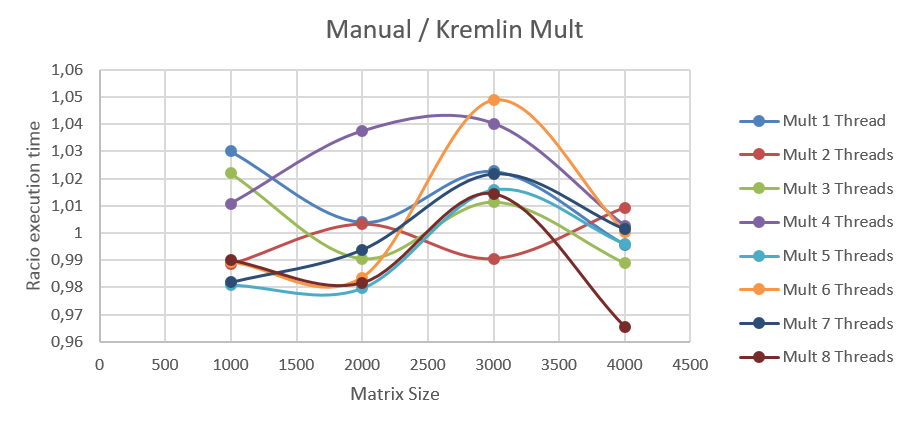
\includegraphics[width=0.8\textwidth]{manualkremlinmul}
		\caption{Dispersion plot that represents the evolution of execution time ratio with the matrix size in function of the number of threads, for the \textit{Mult} algorithm .}
		\label{fig:manualkremlinmul}
	\end{center}
\end{figure}

\begin{figure}[htb]
	\begin{center}
		\leavevmode
		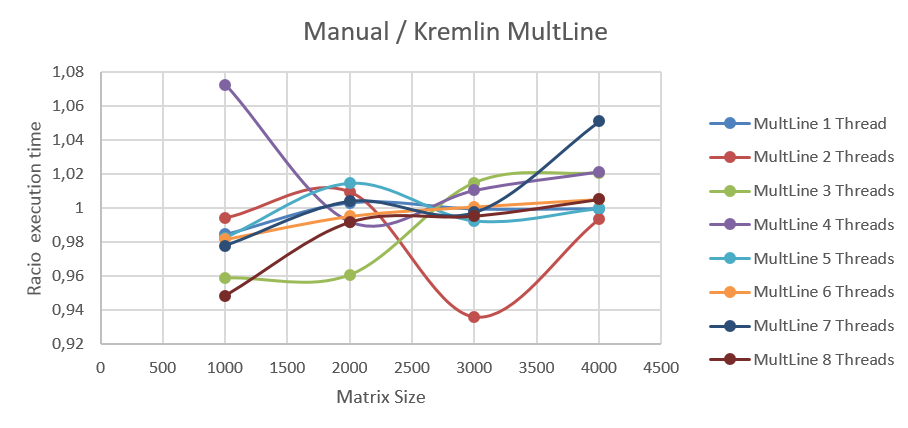
\includegraphics[width=0.9\textwidth]{manualkremlinmuline}
		\caption{Dispersion plot that represents the evolution of execution time ratio with the matrix size in function of the number of threads, for the \textit{MultLine} algorithm.}
		\label{fig:manualkremlinmuline}
	\end{center}
\end{figure}

Confronting Figures~\ref{fig:manualkremlinmul} and~\ref{fig:manualkremlinmuline}, they seemed confusing, messed up, random, and that is partial true because the execution time values from both groups are that close form one another and a slight alteration makes, apparently, an huge impact. It is also partial false because there are patterns in these plots: for each matrix size there is a concentration of lines, meaning that it is not so random and the explanation is that both parallelizations have similar performances. However, and again, the interval value is small.

Trying to se the data in a different angle and perspective to understand if there is any correlation, pattern or relation, these Figures,~\ref{fig:manualkremlinmulthread} and~\ref{fig:manualkremlinmulinethread}, are an unsuccessful attempt of it. The point of these two figures is to understand the variation of execution time ratio with number of threads in function of matrix size, however there is no relation for both cases. So, the number of threads has no direct relation with the execution time ratio in function of the matrix size.


\begin{figure}[htb]
	\begin{center}
		\leavevmode
		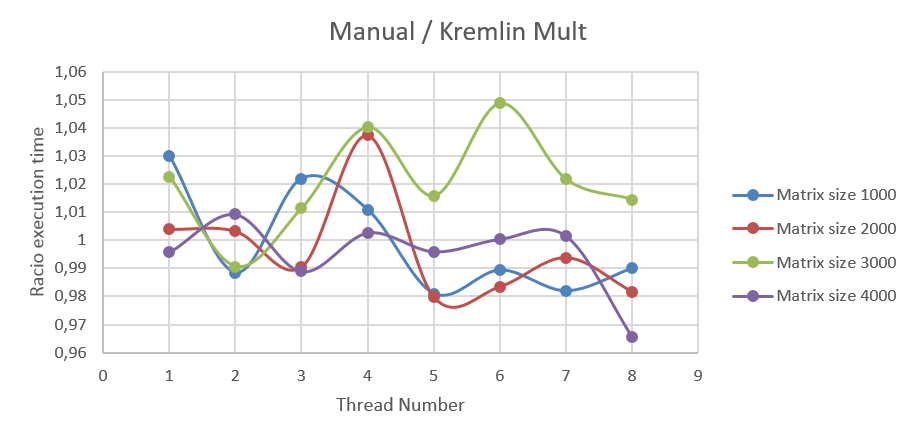
\includegraphics[width=0.8\textwidth]{manualkremlinmulthread}
		\caption{Dispersion plot that represents the evolution of execution time ratio with the number of threads in function of matrix size, for the \textit{Mult} algorithm.}
		\label{fig:manualkremlinmulthread}
	\end{center}
\end{figure}

\begin{figure}[htb]
	\begin{center}
		\leavevmode
		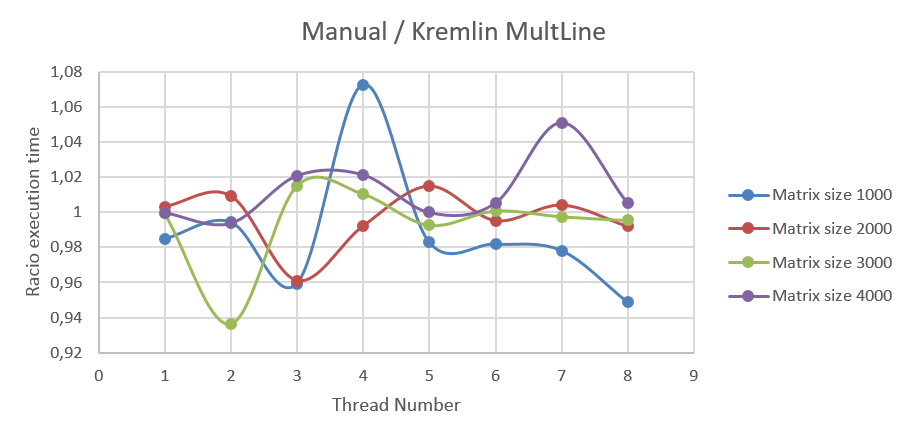
\includegraphics[width=0.9\textwidth]{manualkremlinmulinethread}
		\caption{Dispersion plot that represents the evolution of execution time ratio with the number of threads in function of matrix size, for the \textit{MultLine} algorithm.}
		\label{fig:manualkremlinmulinethread}
	\end{center}
\end{figure}

So far, in this sub sub section, the analysis done is in a general plane. this Figure~\ref{fig:manualkremlin8threads} is about execution time ratio in function of matrix size using eight threads. This specific case was chosen because for both groups, using 8 threads had the best results, as previously mentioned and verified. In the green line is established as a reference: the values under this line mean Kremlin performed better than Manual, and the values above this line mean the opposite. Looking at those values, there is more values under the line than above, meaning that Kremlin group performed better, for both implementations. 
\begin{figure}[htb]
	\begin{center}
		\leavevmode
		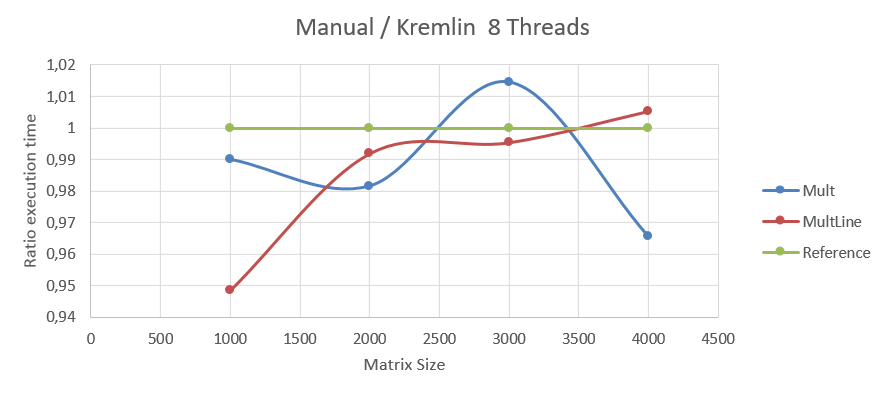
\includegraphics[width=1\textwidth]{manualkremlin8threads}
		\caption{Dispersion plot that represents the evolution of execution time ratio with the matrix size in for 8 threads being used, using \textit{Mult} and \textit{MultLine} algorithms.}
		\label{fig:manualkremlin8threads}
	\end{center}
\end{figure}

